\documentclass[]{article}
\usepackage{lmodern}
\usepackage{amssymb,amsmath}
\usepackage{ifxetex,ifluatex}
\usepackage{fixltx2e} % provides \textsubscript
\ifnum 0\ifxetex 1\fi\ifluatex 1\fi=0 % if pdftex
  \usepackage[T1]{fontenc}
  \usepackage[utf8]{inputenc}
\else % if luatex or xelatex
  \ifxetex
    \usepackage{mathspec}
  \else
    \usepackage{fontspec}
  \fi
  \defaultfontfeatures{Ligatures=TeX,Scale=MatchLowercase}
\fi
% use upquote if available, for straight quotes in verbatim environments
\IfFileExists{upquote.sty}{\usepackage{upquote}}{}
% use microtype if available
\IfFileExists{microtype.sty}{%
\usepackage[]{microtype}
\UseMicrotypeSet[protrusion]{basicmath} % disable protrusion for tt fonts
}{}
\PassOptionsToPackage{hyphens}{url} % url is loaded by hyperref
\usepackage[unicode=true]{hyperref}
\PassOptionsToPackage{usenames,dvipsnames}{color} % color is loaded by hyperref
\hypersetup{
            pdftitle={SC1\_Proj},
            pdfauthor={Alessio},
            colorlinks=true,
            linkcolor=Maroon,
            citecolor=Blue,
            urlcolor=blue,
            breaklinks=true}
\urlstyle{same}  % don't use monospace font for urls
\usepackage[margin=1in]{geometry}
\usepackage{color}
\usepackage{fancyvrb}
\newcommand{\VerbBar}{|}
\newcommand{\VERB}{\Verb[commandchars=\\\{\}]}
\DefineVerbatimEnvironment{Highlighting}{Verbatim}{commandchars=\\\{\}}
% Add ',fontsize=\small' for more characters per line
\usepackage{framed}
\definecolor{shadecolor}{RGB}{248,248,248}
\newenvironment{Shaded}{\begin{snugshade}}{\end{snugshade}}
\newcommand{\KeywordTok}[1]{\textcolor[rgb]{0.13,0.29,0.53}{\textbf{#1}}}
\newcommand{\DataTypeTok}[1]{\textcolor[rgb]{0.13,0.29,0.53}{#1}}
\newcommand{\DecValTok}[1]{\textcolor[rgb]{0.00,0.00,0.81}{#1}}
\newcommand{\BaseNTok}[1]{\textcolor[rgb]{0.00,0.00,0.81}{#1}}
\newcommand{\FloatTok}[1]{\textcolor[rgb]{0.00,0.00,0.81}{#1}}
\newcommand{\ConstantTok}[1]{\textcolor[rgb]{0.00,0.00,0.00}{#1}}
\newcommand{\CharTok}[1]{\textcolor[rgb]{0.31,0.60,0.02}{#1}}
\newcommand{\SpecialCharTok}[1]{\textcolor[rgb]{0.00,0.00,0.00}{#1}}
\newcommand{\StringTok}[1]{\textcolor[rgb]{0.31,0.60,0.02}{#1}}
\newcommand{\VerbatimStringTok}[1]{\textcolor[rgb]{0.31,0.60,0.02}{#1}}
\newcommand{\SpecialStringTok}[1]{\textcolor[rgb]{0.31,0.60,0.02}{#1}}
\newcommand{\ImportTok}[1]{#1}
\newcommand{\CommentTok}[1]{\textcolor[rgb]{0.56,0.35,0.01}{\textit{#1}}}
\newcommand{\DocumentationTok}[1]{\textcolor[rgb]{0.56,0.35,0.01}{\textbf{\textit{#1}}}}
\newcommand{\AnnotationTok}[1]{\textcolor[rgb]{0.56,0.35,0.01}{\textbf{\textit{#1}}}}
\newcommand{\CommentVarTok}[1]{\textcolor[rgb]{0.56,0.35,0.01}{\textbf{\textit{#1}}}}
\newcommand{\OtherTok}[1]{\textcolor[rgb]{0.56,0.35,0.01}{#1}}
\newcommand{\FunctionTok}[1]{\textcolor[rgb]{0.00,0.00,0.00}{#1}}
\newcommand{\VariableTok}[1]{\textcolor[rgb]{0.00,0.00,0.00}{#1}}
\newcommand{\ControlFlowTok}[1]{\textcolor[rgb]{0.13,0.29,0.53}{\textbf{#1}}}
\newcommand{\OperatorTok}[1]{\textcolor[rgb]{0.81,0.36,0.00}{\textbf{#1}}}
\newcommand{\BuiltInTok}[1]{#1}
\newcommand{\ExtensionTok}[1]{#1}
\newcommand{\PreprocessorTok}[1]{\textcolor[rgb]{0.56,0.35,0.01}{\textit{#1}}}
\newcommand{\AttributeTok}[1]{\textcolor[rgb]{0.77,0.63,0.00}{#1}}
\newcommand{\RegionMarkerTok}[1]{#1}
\newcommand{\InformationTok}[1]{\textcolor[rgb]{0.56,0.35,0.01}{\textbf{\textit{#1}}}}
\newcommand{\WarningTok}[1]{\textcolor[rgb]{0.56,0.35,0.01}{\textbf{\textit{#1}}}}
\newcommand{\AlertTok}[1]{\textcolor[rgb]{0.94,0.16,0.16}{#1}}
\newcommand{\ErrorTok}[1]{\textcolor[rgb]{0.64,0.00,0.00}{\textbf{#1}}}
\newcommand{\NormalTok}[1]{#1}
\usepackage{longtable,booktabs}
% Fix footnotes in tables (requires footnote package)
\IfFileExists{footnote.sty}{\usepackage{footnote}\makesavenoteenv{long table}}{}
\usepackage{graphicx,grffile}
\makeatletter
\def\maxwidth{\ifdim\Gin@nat@width>\linewidth\linewidth\else\Gin@nat@width\fi}
\def\maxheight{\ifdim\Gin@nat@height>\textheight\textheight\else\Gin@nat@height\fi}
\makeatother
% Scale images if necessary, so that they will not overflow the page
% margins by default, and it is still possible to overwrite the defaults
% using explicit options in \includegraphics[width, height, ...]{}
\setkeys{Gin}{width=\maxwidth,height=\maxheight,keepaspectratio}
\IfFileExists{parskip.sty}{%
\usepackage{parskip}
}{% else
\setlength{\parindent}{0pt}
\setlength{\parskip}{6pt plus 2pt minus 1pt}
}
\setlength{\emergencystretch}{3em}  % prevent overfull lines
\providecommand{\tightlist}{%
  \setlength{\itemsep}{0pt}\setlength{\parskip}{0pt}}
\setcounter{secnumdepth}{0}
% Redefines (sub)paragraphs to behave more like sections
\ifx\paragraph\undefined\else
\let\oldparagraph\paragraph
\renewcommand{\paragraph}[1]{\oldparagraph{#1}\mbox{}}
\fi
\ifx\subparagraph\undefined\else
\let\oldsubparagraph\subparagraph
\renewcommand{\subparagraph}[1]{\oldsubparagraph{#1}\mbox{}}
\fi

% set default figure placement to htbp
\makeatletter
\def\fps@figure{htbp}
\makeatother

\usepackage{algorithm2e}
\usepackage{amsmath}
\usepackage{bm}

\title{SC1\_Proj}
\author{Alessio}
\date{}

\begin{document}
\maketitle

\newcommand{\vect}[1]{\boldsymbol{\mathbf{#1}}}
\newcommand{\vbeta}{\vect{\beta}}
\newcommand{\vx}{\vect{x}}
\newcommand{\vy}{\vect{y}}
\newcommand{\vzero}{\vect{0}}
\newcommand{\vSigma}{\vect{\Sigma}}
\newcommand{\vtheta}{\vect{\theta}}
\newcommand{\uniform}{\mathcal{U}(0, 1)}






\section{Introduction}\label{introduction}

One of the most common types of cancer diagnosed in women is breast
cancer. There are multiple tests that people are subjected to, but one
of the most indicative ones is fine needle aspiration which involes
extracting a sample of cells to be examined under a microscope. Multiple
numerical metrics are computed from the obtained images. The aim is to
use the extracted metrics to make accurate diagnoses.

The dataset consists of \(569\) images which have been processed as
described and a total of \(30\) variables have been computed for each
observation. The aim of this report is to implement a number of
classification algorithms, use them to obtain predictions, and compare
their performances.

\section{Exploratory analysis}\label{exploratory-analysis}

We begin by exploring the data to gain some understanding of the
features and their relationships to inform further work. We do the
majority of the data manipulation and analysis within this report using
the tidyverse library. We begin by loading the data as a tibble:

\begin{Shaded}
\begin{Highlighting}[]
\NormalTok{data <-}\StringTok{ }\KeywordTok{read_csv}\NormalTok{(}\StringTok{"../data/data.csv"}\NormalTok{)}
\end{Highlighting}
\end{Shaded}

After renaming some variables to some more manageable variables we next
have to ensure the hygiene of our data. Through manual inspection it is
clear that our data is already in the tidy data format so all that
remains is to see if any corrupted data is present:

\begin{Shaded}
\begin{Highlighting}[]
\KeywordTok{colSums}\NormalTok{(}\KeywordTok{is.na}\NormalTok{(data))}
\end{Highlighting}
\end{Shaded}

\begin{verbatim}
##           id    diagnosis     radius_m    texture_m      perim_m       area_m 
##            0            0            0            0            0            0 
##     smooth_m    compact_m     concav_m  concav_pt_m   symmetry_m   frac_dim_m 
##            0            0            0            0            0            0 
##    radius_se   texture_se     perim_se      area_se    smooth_se   compact_se 
##            0            0            0            0            0            0 
##    concav_se concav_pt_se  symmetry_se  frac_dim_se     radius_w    texture_w 
##            0            0            0            0            0            0 
##      perim_w       area_w     smooth_w    compact_w     concav_w  concav_pt_w 
##            0            0            0            0            0            0 
##   symmetry_w   frac_dim_w          X33 
##            0            0          569
\end{verbatim}

From this we can see that the feature parsed as \texttt{X33} is not
present for any observation and therefore can be removed without any
difficulties using \texttt{dplyr}

\begin{Shaded}
\begin{Highlighting}[]
\NormalTok{data }\OperatorTok
\StringTok{  }\NormalTok{dplyr}\OperatorTok{::}\KeywordTok{select}\NormalTok{(}\OperatorTok{-}\KeywordTok{c}\NormalTok{(X33))}
\end{Highlighting}
\end{Shaded}

In order to make the data easier to work with we also need to set the
response, the diagnosis of the patient, to be a factor.

\begin{Shaded}
\begin{Highlighting}[]
\NormalTok{data }\OperatorTok\StringTok{ }\KeywordTok{mutate_at}\NormalTok{(}\KeywordTok{vars}\NormalTok{(diagnosis), factor)}
\end{Highlighting}
\end{Shaded}

The next step before analysing the data is to produce a test/train split
in order to evaluate how well our models and methods will generalise
which we can do again using \texttt{dplyr}. We choose an 80/20
train/test split.

\begin{Shaded}
\begin{Highlighting}[]
\NormalTok{train <-}\StringTok{ }\NormalTok{data }\OperatorTok\StringTok{ }\KeywordTok{sample_frac}\NormalTok{(}\FloatTok{0.8}\NormalTok{)}
\NormalTok{test <-}\StringTok{ }\KeywordTok{anti_join}\NormalTok{(data, train, }\DataTypeTok{by =} \StringTok{"id"}\NormalTok{)}
\end{Highlighting}
\end{Shaded}

We also remove the labels and store them elsewhere so that we have the
raw data input to analyse.

\begin{Shaded}
\begin{Highlighting}[]
\NormalTok{id_train <-}\StringTok{ }\NormalTok{train}\OperatorTok{$}\NormalTok{id}
\NormalTok{id_test <-}\StringTok{ }\NormalTok{test}\OperatorTok{$}\NormalTok{id}

\NormalTok{data }\OperatorTok
\StringTok{  }\NormalTok{dplyr}\OperatorTok{::}\KeywordTok{select}\NormalTok{(}\OperatorTok{-}\KeywordTok{c}\NormalTok{(id))}
\NormalTok{train }\OperatorTok
\StringTok{  }\NormalTok{dplyr}\OperatorTok{::}\KeywordTok{select}\NormalTok{(}\OperatorTok{-}\KeywordTok{c}\NormalTok{(id))}
\NormalTok{test }\OperatorTok
\StringTok{  }\NormalTok{dplyr}\OperatorTok{::}\KeywordTok{select}\NormalTok{(}\OperatorTok{-}\KeywordTok{c}\NormalTok{(id))}
\end{Highlighting}
\end{Shaded}

Before continuing with our analysis we need to make sure that the
train/test split is representative of the entire data. Below is a plot
of the class distribution in the training set on the left and the test
set on the right. As can be seen these are fairly even and therefore
this split is suitable for analysis.
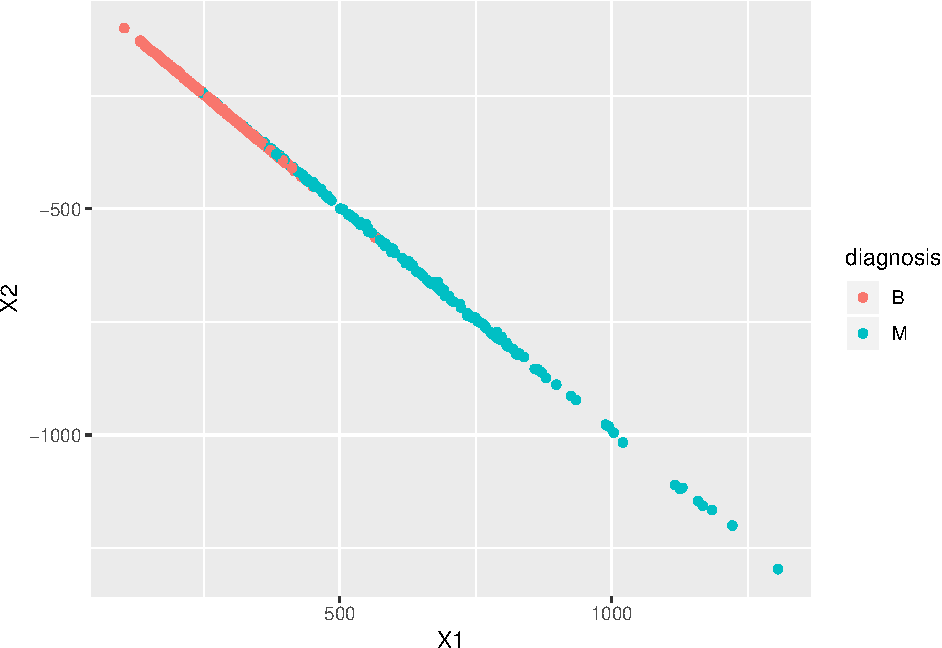
\includegraphics{final_submission_files/figure-latex/unnamed-chunk-11-1.pdf}

We now want to try and discover if our data has any exploitable
structure that we can use for classification. We can examine the density
plots of each feature for each class against each other to see if there
are features which have substantially different plots.

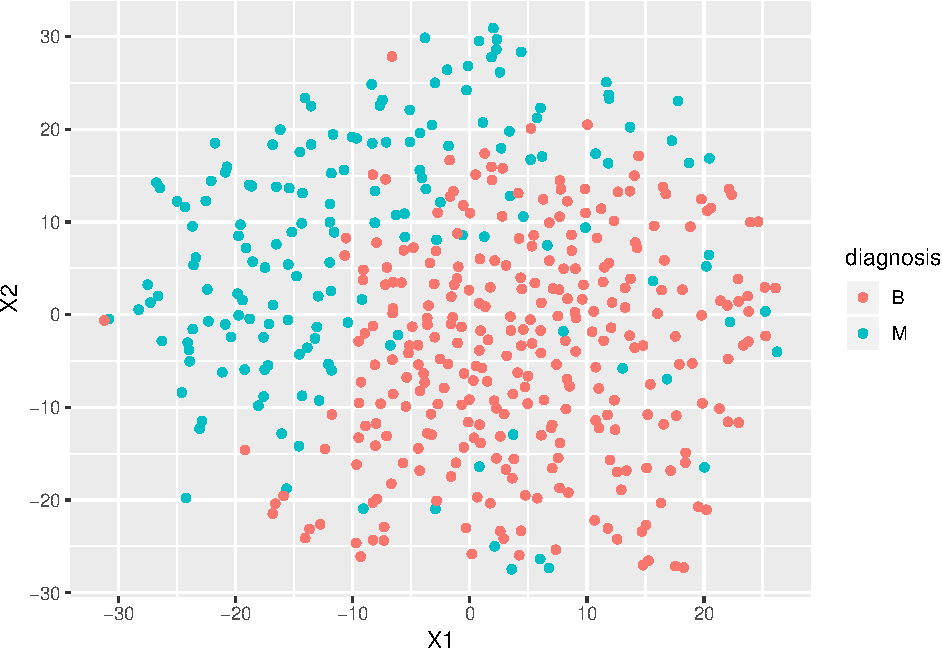
\includegraphics{final_submission_files/figure-latex/unnamed-chunk-12-1.pdf}

From these plots above we can see that many of the features are, from
visual, inspection, approximately normal. Whilst this is not conclusive
as per a test however this may justify some techniques for
classification which rely on normality of the features (as in the choice
of naive bayes below).

Many of the features display little difference in densities between
classes however several of the features display noticeable difference
which is promising for modelling.

The final plot we want to do is to check the pairwise correlations
betwee all pairs of features.
\includegraphics{final_submission_files/figure-latex/unnamed-chunk-13-1.pdf}

This plot shows that a large number of our features are highly
correlated which gives us some indication that we can perhaps predict
some features from others and reduce the dimension of the data we are
working with. Now that we have established that there appears to be some
structure within our data and that there appears to be more important
variables we can move on with an attempt to reduce the dimensionality of
our data. \newpage
\# Dimensionality Reduction and Feature Selection

\subsection{PCA}\label{pca}

For data of a non-trivial dimensionality it can be difficult to know
where to begin with the modelling process as we may not have an
intuitive idea of the underlying structure in our code. One such method
of visualising the data in a lower space is principal component analysis
(PCA). PCA aims to produce a set of linearly uncorrelated variables from
our original set of variables of a reduced size. It does this by first
taking the dataset represented as a matrix:

\[
X = \begin{pmatrix}
x_{1}^{T} \\
\vdots \\
x_{2}^{T}
\end{pmatrix}
\] then we form a matrix normalised by the standard score by subtracting
the column means from every column and dividing every column by the
standard deviation for that column as in:

\begin{Shaded}
\begin{Highlighting}[]
\NormalTok{normalise_z <-}\StringTok{ }\ControlFlowTok{function}\NormalTok{(X) \{}
\NormalTok{  mean_cols <-}\StringTok{ }\KeywordTok{colMeans}\NormalTok{(X)}
\NormalTok{  sd_cols <-}\StringTok{ }\KeywordTok{apply}\NormalTok{(X, }\DecValTok{2}\NormalTok{, sd)}
\NormalTok{  mean_normalised_X <-}\StringTok{ }\KeywordTok{t}\NormalTok{(}\KeywordTok{apply}\NormalTok{(X, }\DecValTok{1}\NormalTok{, }\ControlFlowTok{function}\NormalTok{(x) \{}
\NormalTok{    x }\OperatorTok{-}\StringTok{ }\NormalTok{mean_cols}
\NormalTok{  \}))}
\NormalTok{  normalised_X <-}\StringTok{ }\KeywordTok{t}\NormalTok{(}\KeywordTok{apply}\NormalTok{(mean_normalised_X, }\DecValTok{1}\NormalTok{, }\ControlFlowTok{function}\NormalTok{(x) \{}
\NormalTok{    x }\OperatorTok{/}\StringTok{ }\NormalTok{sd_cols}
\NormalTok{  \}))}
  \KeywordTok{return}\NormalTok{(normalised_X)}
\NormalTok{\}}
\end{Highlighting}
\end{Shaded}

Giving us: \[
Z = \begin{pmatrix} 
\frac{x_{11} - \mu_{1}}{\sigma_{1}} & ... & \frac{x_{1d} - \mu_{d}}{\sigma{d}} \\
\vdots & \vdots & \vdots \\
\frac{x_{n1} - \mu_{1}}{\sigma_{1}} & ... & \frac{x_{nd} - \mu_{d}}{\sigma{d}} \\
\end{pmatrix}
\] Multiplying this by its transpose gives us the correlation matrix
where the entry \(\rho_{ij}\) is the correlation between observation
\(i\) and observation \(j\). We can take the eigendecomposition of this
matrix product to give us:

\[
Z^{T}Z = P \,\Sigma^{-1}P^{T}
\] Where we assume that the diagonal \(\Sigma\) is ordered by size. The
eigenvectors corresponding to the largest eigenvalues represent the
combinations of features which account for the highest variance. If we
wish to visualise at dimension \(k < d\) we can simply take the top
\(k\) eigenvectors as a matrix and multiply our data by this visualise
our data in the reduced space. Code that does this can be found below.

\begin{Shaded}
\begin{Highlighting}[]
\NormalTok{pca <-}\StringTok{ }\ControlFlowTok{function}\NormalTok{(X, number_components_keep) \{}
\NormalTok{  normalised_X <-}\StringTok{ }\KeywordTok{normalise_z}\NormalTok{(X)}

\NormalTok{  corr_mat <-}\StringTok{ }\KeywordTok{t}\NormalTok{(normalised_X) }\OperatorTok\StringTok{ }\NormalTok{normalised_X}

\NormalTok{  eigenvectors <-}\StringTok{ }\KeywordTok{eigen}\NormalTok{(corr_mat, }\DataTypeTok{symmetric =} \OtherTok{TRUE}\NormalTok{)}\OperatorTok{$}\NormalTok{vectors}

\NormalTok{  reduced_data <-}\StringTok{ }\NormalTok{X }\OperatorTok\StringTok{ }\NormalTok{eigenvectors[, }\DecValTok{1}\OperatorTok{:}\NormalTok{number_components_keep]}
\NormalTok{  relevant_eigs <-}\StringTok{ }\NormalTok{eigenvectors[, }\DecValTok{1}\OperatorTok{:}\NormalTok{number_components_keep]}
\NormalTok{  returnds <-}\StringTok{ }\KeywordTok{list}\NormalTok{(reduced_data, relevant_eigs)}
  \KeywordTok{names}\NormalTok{(returnds) <-}\StringTok{ }\KeywordTok{c}\NormalTok{(}\StringTok{"reduced_data"}\NormalTok{, }\StringTok{"reduction_matrix"}\NormalTok{)}
  \KeywordTok{return}\NormalTok{(returnds)}
\NormalTok{\}}
\end{Highlighting}
\end{Shaded}

When applying this to the dataset and keeping 2 components the following
plot results:

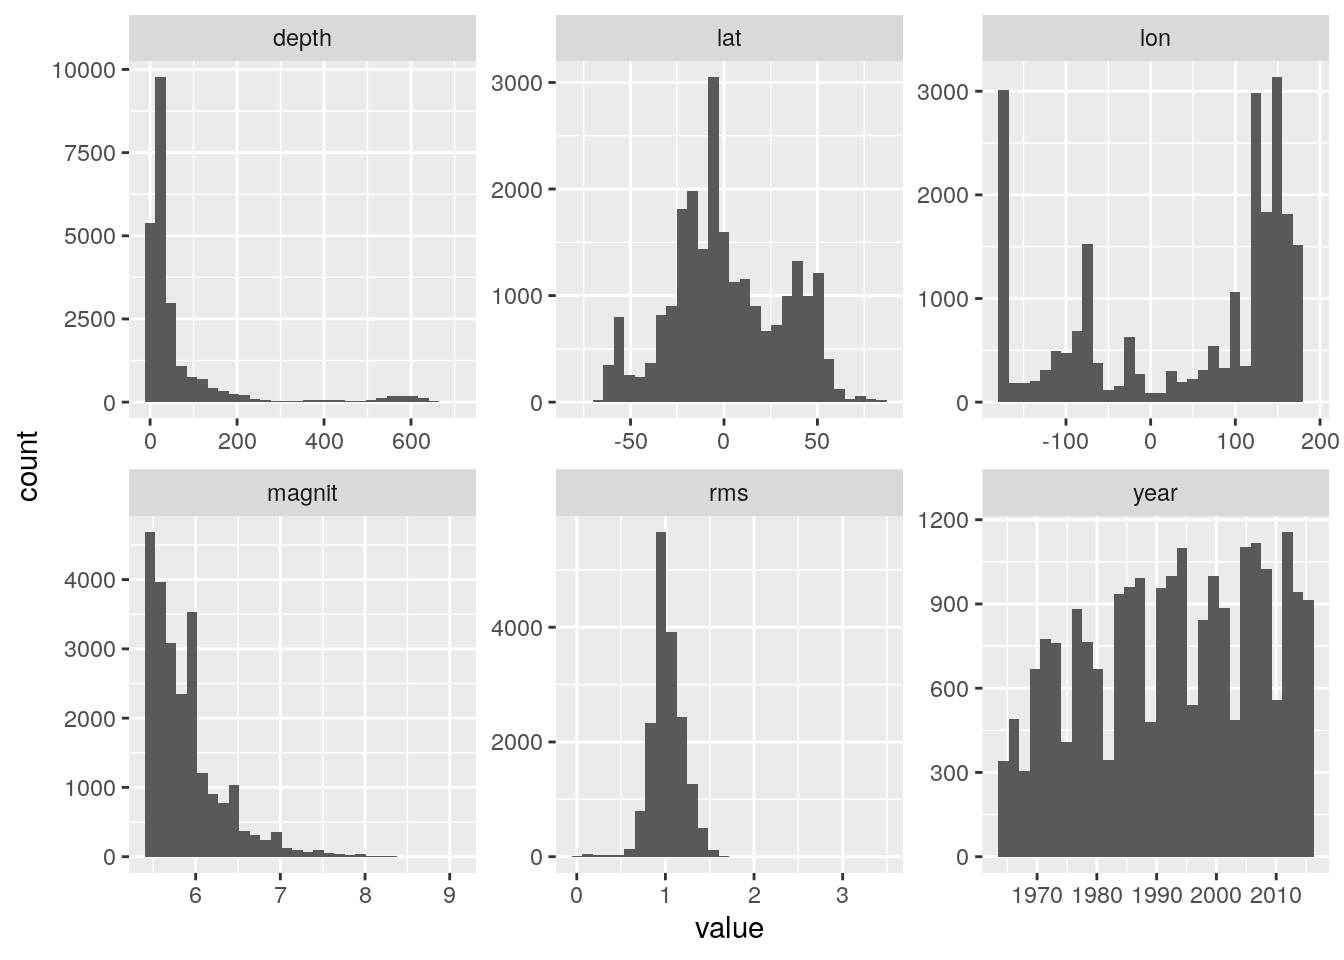
\includegraphics{final_submission_files/figure-latex/unnamed-chunk-16-1.pdf}

As we can see from this plot there is clearly some structure within the
data that we can exploit for classification.

\newpage

\section{Classification}\label{classification}

add list of methods+measure

\subsection{SVM}\label{svm}

From the application of PCA to the dataset we can see that, after
reducing to 2 dimensions, the data appears to be almost linearly
separable. Given this, an appropriate method of classifying the data
would be to apply a soft-margin SVM to the reduced dimension data.
Soft-margin SVMs solve the problem of classifying non-separable data by
permitting a certain number of points to be incorrectly classifed
however the number and the amount they violate the constraints by must
be as small as possible. After manipulating the reformulated
optimisation problem we end up with the optimisation problem \[
\underset{\lambda}{\text{min}} \, \frac{\overline{\lambda}X X^{T}\overline{\lambda^{T}}}{4}
+ \lambda^{T}\bm{1}
\] \[
\text{such that } 0 \leq \lambda_{i} \leq C
\] \[
\text{and } \sum\limits_{i}^{n} \lambda_{i}y_{i} = 0
\]

where \[
X = \begin{pmatrix}
x_{1}^{T} \\
\vdots \\
x_{n}^{T}
\end{pmatrix} \text{ and } 
\overline{\lambda} = [\lambda_{1} \cdot y_{i}, ... , \lambda_{n} \cdot y_{n}] \text{ and } \bm{1} = [1, ..., 1] \in \mathbb{R^{n}}
\] For some predefined \(C\). This is a quadratic programming problem
with linear constraints which can be solved using the R package
\texttt{quadprog}with the function \texttt{solve.QP}. From its
documentation, this function can solve (for \(b\)) problems in the form
\(\underset{b}{\text{min}}(-d^{T}b + \frac{1}{2} b^{T}Db)\) with the
constraints that \(A^{T} b \geq b_0\). By transforming the above problem
into this format we can implement soft-margin SVM using the following
code

\begin{Shaded}
\begin{Highlighting}[]
\NormalTok{train_soft_svm <-}\StringTok{ }\ControlFlowTok{function}\NormalTok{(X, y, C) \{}
  
\NormalTok{  num_observation <-}\StringTok{ }\KeywordTok{nrow}\NormalTok{(X)}
\NormalTok{  dim_num <-}\StringTok{ }\KeywordTok{ncol}\NormalTok{(X)}

\NormalTok{  Dmat2 <-}\StringTok{ }\KeywordTok{diag}\NormalTok{(y) }\OperatorTok{*}\StringTok{ }\NormalTok{X }\OperatorTok\StringTok{ }\KeywordTok{t}\NormalTok{(X) }\OperatorTok\StringTok{ }\KeywordTok{diag}\NormalTok{(y)}
  \KeywordTok{diag}\NormalTok{(Dmat2) <-}\StringTok{ }\KeywordTok{diag}\NormalTok{(Dmat2) }\OperatorTok{+}\StringTok{ }\FloatTok{1e-6}
\NormalTok{  dv2 <-}\StringTok{ }\KeywordTok{rep}\NormalTok{(}\DecValTok{1}\NormalTok{, num_observation)}
  
\NormalTok{  A2 <-}\StringTok{ }\KeywordTok{rbind}\NormalTok{( y,}\KeywordTok{diag}\NormalTok{(num_observation)) }
\NormalTok{  A2 <-}\StringTok{ }\KeywordTok{rbind}\NormalTok{(A2, }\OperatorTok{-}\DecValTok{1}\OperatorTok{*}\KeywordTok{diag}\NormalTok{(num_observation))}
  
\NormalTok{  bv2 <-}\StringTok{ }\KeywordTok{c}\NormalTok{(}\KeywordTok{c}\NormalTok{(}\DecValTok{0}\NormalTok{), }\KeywordTok{rep}\NormalTok{(}\DecValTok{0}\NormalTok{, num_observation), }\KeywordTok{rep}\NormalTok{(}\OperatorTok{-}\NormalTok{C, num_observation) )}
\NormalTok{  model <-}\StringTok{ }\KeywordTok{solve.QP}\NormalTok{(Dmat2, dv2, }\KeywordTok{t}\NormalTok{(A2), bv2, }\DataTypeTok{meq =} \DecValTok{1}\NormalTok{) }
\NormalTok{\}}
\end{Highlighting}
\end{Shaded}

In order to recover \(w\) and \(b\) from \(\lambda\) we use the
relationship \[
w = \sum\limits_{i=0}^{n-1}\lambda_{i}x_{i}^{T}y_{i}
\] and \[
b = \text{mean}(\sum\limits_{i=0}^{k} y_{i} - w \cdot x_{i}) \, . \, \forall \, i . 0 < \lambda_{i} < C
\]

Which can be made as functions in R as so:

\begin{Shaded}
\begin{Highlighting}[]
\NormalTok{calculate_b <-}\StringTok{ }\ControlFlowTok{function}\NormalTok{(w, X, y, a, C) \{}
\NormalTok{  ks <-}\StringTok{ }\KeywordTok{sapply}\NormalTok{(a, }\ControlFlowTok{function}\NormalTok{(x) \{}
    \KeywordTok{return}\NormalTok{(x }\OperatorTok{>}\StringTok{ }\DecValTok{0} \OperatorTok{&&}\StringTok{ }\NormalTok{x }\OperatorTok{<}\StringTok{ }\NormalTok{C)}
\NormalTok{  \})}
\NormalTok{  indices <-}\StringTok{ }\KeywordTok{which}\NormalTok{(ks)}
\NormalTok{  sum_bs <-}\StringTok{ }\DecValTok{0}
  \ControlFlowTok{for}\NormalTok{ (i }\ControlFlowTok{in}\NormalTok{ indices) \{}
\NormalTok{    sum_bs <-}\StringTok{ }\NormalTok{sum_bs }\OperatorTok{+}\StringTok{ }\NormalTok{(y[i] }\OperatorTok{-}\StringTok{ }\NormalTok{w }\OperatorTok\StringTok{ }\NormalTok{X[i, ])}
\NormalTok{  \}}
  \KeywordTok{return}\NormalTok{(sum_bs }\OperatorTok{/}\StringTok{ }\KeywordTok{length}\NormalTok{(indices))}
\NormalTok{\}}


\NormalTok{recover_w <-}\StringTok{ }\ControlFlowTok{function}\NormalTok{(a, y, X) \{}
  \KeywordTok{colSums}\NormalTok{(}\KeywordTok{diag}\NormalTok{(a) }\OperatorTok\StringTok{ }\KeywordTok{diag}\NormalTok{(y) }\OperatorTok\StringTok{ }\NormalTok{X)}
\NormalTok{\}}
\end{Highlighting}
\end{Shaded}

From the parameters we can recover the equation of the line
corresopnding the decision boundary which can later be used for plotting

\begin{Shaded}
\begin{Highlighting}[]
\NormalTok{soft_margin_svm_plotter <-}\StringTok{ }\ControlFlowTok{function}\NormalTok{(w, b) \{}
\NormalTok{  plotter <-}\StringTok{ }\ControlFlowTok{function}\NormalTok{(x) \{}
    \KeywordTok{return}\NormalTok{(}\DecValTok{1} \OperatorTok{/}\StringTok{ }\NormalTok{w[}\DecValTok{2}\NormalTok{] }\OperatorTok{*}\StringTok{ }\OperatorTok{-}\NormalTok{(b }\OperatorTok{+}\StringTok{ }\NormalTok{(w[}\DecValTok{1}\NormalTok{] }\OperatorTok{*}\StringTok{ }\KeywordTok{as.numeric}\NormalTok{(x))))}
\NormalTok{  \}}
  \KeywordTok{return}\NormalTok{(plotter)}
\NormalTok{\}}
\end{Highlighting}
\end{Shaded}

TODO: prediction function

We are now able to define a function which first embeds the vector in
the reduced space and then predicts the class based upon the prediction
function produced by the parameters found by the SVM. Below is code that
will do the following based upon a package written for this assignment
found
\href{https://github.com/alessio-b-zak/sc1-svm-example-package}{here}

\begin{Shaded}
\begin{Highlighting}[]
\NormalTok{model <-}\StringTok{ }\KeywordTok{svm}\NormalTok{(}
  \DataTypeTok{X =}\NormalTok{ pca_result}\OperatorTok{$}\NormalTok{reduced_data,}
  \DataTypeTok{classes =}\NormalTok{ numeric_training_labels,}
  \DataTypeTok{C =} \DecValTok{100000}\NormalTok{, }\DataTypeTok{margin_type =} \StringTok{"soft"}\NormalTok{,}
  \DataTypeTok{kernel_function =}\NormalTok{ linear_kernel,}
  \DataTypeTok{feature_map =}\NormalTok{ linear_basis_function}
\NormalTok{)}


\NormalTok{reduced_prediction_fn <-}\StringTok{ }\NormalTok{model}\OperatorTok{$}\NormalTok{prediction_function}

\NormalTok{pca_reduced_prediction_fn <-}\StringTok{ }\ControlFlowTok{function}\NormalTok{(x) \{}
\NormalTok{  p <-}\StringTok{ }\NormalTok{x }\OperatorTok\StringTok{ }\NormalTok{pca_result}\OperatorTok{$}\NormalTok{reduction_matrix}
  \KeywordTok{reduced_prediction_fn}\NormalTok{(}\KeywordTok{t}\NormalTok{(p))}
\NormalTok{\}}
\end{Highlighting}
\end{Shaded}

\begin{Shaded}
\begin{Highlighting}[]
\NormalTok{pca_reduced_test_data <-}\StringTok{ }\KeywordTok{t}\NormalTok{(}\KeywordTok{apply}\NormalTok{(}\KeywordTok{as.matrix}\NormalTok{(test_data), }\DecValTok{1}\NormalTok{, }\ControlFlowTok{function}\NormalTok{(x) x }\OperatorTok
\StringTok{                                   }\NormalTok{pca_result}\OperatorTok{$}\NormalTok{reduction_matrix))}
\end{Highlighting}
\end{Shaded}

When running the trained SVM prediction functio on the test set we
achieve 86.8421053 \%. We can plot this code as below

\includegraphics{final_submission_files/figure-latex/unnamed-chunk-25-1.pdf}

\begin{Shaded}
\begin{Highlighting}[]
\NormalTok{confusion_plot <-}\StringTok{ }\ControlFlowTok{function}\NormalTok{(actual, predicted, }\DataTypeTok{method=}\StringTok{''}\NormalTok{) \{}
\NormalTok{  confusion_matrix <-}\StringTok{ }\KeywordTok{as.data.frame}\NormalTok{(}\KeywordTok{table}\NormalTok{(actual, predicted))}
\NormalTok{  g <-}\StringTok{ }\KeywordTok{ggplot}\NormalTok{(confusion_matrix, }\KeywordTok{aes}\NormalTok{(}\DataTypeTok{x =}\NormalTok{ actual, }\DataTypeTok{y =}\NormalTok{ predicted)) }\OperatorTok{+}
\StringTok{    }\KeywordTok{geom_tile}\NormalTok{(}\KeywordTok{aes}\NormalTok{(}\DataTypeTok{fill =}\NormalTok{ Freq)) }\OperatorTok{+}
\StringTok{    }\KeywordTok{geom_text}\NormalTok{(}\KeywordTok{aes}\NormalTok{(}\DataTypeTok{label =} \KeywordTok{sprintf}\NormalTok{(}\StringTok{"%1.0f"}\NormalTok{, Freq)), }\DataTypeTok{color =} \StringTok{"white"}\NormalTok{, }\DataTypeTok{fontface =} \StringTok{"bold"}\NormalTok{) }\OperatorTok{+}
\StringTok{    }\KeywordTok{labs}\NormalTok{(}\DataTypeTok{x =} \StringTok{"Actual"}\NormalTok{, }\DataTypeTok{y =} \StringTok{"Predicted"}\NormalTok{,}\DataTypeTok{title=}\NormalTok{method) }\OperatorTok{+}
\StringTok{    }\KeywordTok{theme_minimal}\NormalTok{()}\OperatorTok{+}
\StringTok{    }\KeywordTok{theme}\NormalTok{(}\DataTypeTok{legend.position =} \StringTok{'none'}\NormalTok{,}
          \DataTypeTok{plot.title =} \KeywordTok{element_text}\NormalTok{(}\DataTypeTok{hjust=}\FloatTok{0.5}\NormalTok{))}
  \KeywordTok{return}\NormalTok{(g)}
\NormalTok{\}}
\end{Highlighting}
\end{Shaded}

\begin{Shaded}
\begin{Highlighting}[]
\KeywordTok{confusion_plot}\NormalTok{(numeric_test_labels,pred_svm,}\StringTok{'SVM'}\NormalTok{)}
\end{Highlighting}
\end{Shaded}

\includegraphics{final_submission_files/figure-latex/unnamed-chunk-27-1.pdf}

\newpage

\section{Naive Bayes}\label{naive-bayes}

\subsection{Mathematical setting}\label{mathematical-setting}

Let \(y\) be the class label that we want to assign to an observation
\(\boldsymbol{x}=(x_1,\cdots x_d)\), where \(x_1,\cdots x_d\) are the
features. The probability of an observation having label \(y\) is given
by Bayes rule,

\begin{align*}
P(y|x_1,\cdots,x_d)&=\frac{P(x_1,\cdots,x_d|y_k)P(y)}{P(x_1,\cdots,x_d)}\\
&\propto P(x_1,\cdots,x_d|y_k)P(y).
\end{align*}

The prior class probability \(P(y)\) can be easily obtained by the
proportion of observation that are in the given class.

The main assumption is that every feature is conditionally independent
given the class label \(y\). The reason why this classifier is called
\emph{naive} is that very often this assumption is not actually
realistic.

This assumption simplifies the posterior to
\[P(y|x_1,\cdots,x_d) \propto P(y)\prod_{i=1}^d P(x_i|y).\] There are
various types of Naive Bayes classifiers based on the type of features.
In our case, since we have continuous variables we assume that all
features are normally distributed. Therefore, the conditional
probabilities can be calculated as
\[P(x_i|y)=\frac{1}{\sqrt{2\pi\sigma_y^2}}exp\left(-\frac{(x_i-\mu_y)^2}{2\sigma_y^2}\right)\]

Finally, to assign the class to an observation we use the Maximum A
Posteriori decision rule. For every observation, we pick the class the
has the highest probability
\[y=\underset{y}{\text{argmax}}P(y)\prod_{i=1}^dP(x_i|y).\]

\subsection{Implementation}\label{implementation}

\emph{Here are some code snippets just to illustrate how these
theoretical aspects are implemented. The full code can be found in the
package.}

The observations are stored as rows in \(X\) and the corresponding class
labels are entires in the column matrix \(y\).

First we calculate the prior class probabilities based on the number of
observations in each class.

\begin{Shaded}
\begin{Highlighting}[]
\NormalTok{n <-}\StringTok{ }\KeywordTok{dim}\NormalTok{(X)[}\DecValTok{1}\NormalTok{]}
\NormalTok{d <-}\StringTok{ }\KeywordTok{dim}\NormalTok{(X)[}\DecValTok{2}\NormalTok{]}
\NormalTok{classes <-}\StringTok{ }\KeywordTok{sort}\NormalTok{(}\KeywordTok{unique}\NormalTok{(y)[, }\DecValTok{1}\NormalTok{])}
\NormalTok{k <-}\StringTok{ }\KeywordTok{length}\NormalTok{(classes)}

\NormalTok{prior <-}\StringTok{ }\KeywordTok{rep}\NormalTok{(}\DecValTok{0}\NormalTok{, k)}
\ControlFlowTok{for}\NormalTok{ (i }\ControlFlowTok{in} \DecValTok{1}\OperatorTok{:}\NormalTok{k) \{}
\NormalTok{  prior[i] <-}\StringTok{ }\KeywordTok{sum}\NormalTok{(y }\OperatorTok{==}\StringTok{ }\NormalTok{classes[i]) }\OperatorTok{/}\StringTok{ }\NormalTok{n}
\NormalTok{\}}
\end{Highlighting}
\end{Shaded}

Then we create an array of the mean and sd of the data split by clasess
and features.

\begin{Shaded}
\begin{Highlighting}[]
\NormalTok{summaries <-}\StringTok{ }\KeywordTok{array}\NormalTok{(}\KeywordTok{rep}\NormalTok{(}\DecValTok{1}\NormalTok{, d }\OperatorTok{*}\StringTok{ }\NormalTok{k }\OperatorTok{*}\StringTok{ }\DecValTok{2}\NormalTok{), }\DataTypeTok{dim =} \KeywordTok{c}\NormalTok{(k, d, }\DecValTok{2}\NormalTok{))}
\ControlFlowTok{for}\NormalTok{ (i }\ControlFlowTok{in} \DecValTok{1}\OperatorTok{:}\NormalTok{k) \{}
\NormalTok{  X_k <-}\StringTok{ }\NormalTok{X[}\KeywordTok{which}\NormalTok{(y }\OperatorTok{==}\StringTok{ }\NormalTok{(i }\OperatorTok{-}\StringTok{ }\DecValTok{1}\NormalTok{)), ]}
\NormalTok{  summaries[i, , }\DecValTok{1}\NormalTok{] <-}\StringTok{ }\KeywordTok{apply}\NormalTok{(X_k, }\DecValTok{2}\NormalTok{, mean)}
\NormalTok{  summaries[i, , }\DecValTok{2}\NormalTok{] <-}\StringTok{ }\KeywordTok{apply}\NormalTok{(X_k, }\DecValTok{2}\NormalTok{, sd)}
\NormalTok{\}}
\end{Highlighting}
\end{Shaded}

Finally, the predictions are obtained by taking the largest posterior
class probability. Note that in order to avoid underflow, we take the
maximum of the \emph{log} posterior class probabilities.

\begin{Shaded}
\begin{Highlighting}[]
\NormalTok{probs <-}\StringTok{ }\KeywordTok{matrix}\NormalTok{(}\KeywordTok{rep}\NormalTok{(}\DecValTok{0}\NormalTok{, n }\OperatorTok{*}\StringTok{ }\NormalTok{k), }\DataTypeTok{nrow =}\NormalTok{ n)}
\ControlFlowTok{for}\NormalTok{ (obs }\ControlFlowTok{in} \DecValTok{1}\OperatorTok{:}\NormalTok{n) \{}
  \ControlFlowTok{for}\NormalTok{ (class }\ControlFlowTok{in} \DecValTok{1}\OperatorTok{:}\NormalTok{k) \{}
\NormalTok{    class_prob <-}\StringTok{ }\KeywordTok{log}\NormalTok{(prior[class])}
    \ControlFlowTok{for}\NormalTok{ (feat }\ControlFlowTok{in} \DecValTok{1}\OperatorTok{:}\NormalTok{d) \{}
\NormalTok{      mu <-}\StringTok{ }\NormalTok{summaries[class, feat, }\DecValTok{1}\NormalTok{]}
\NormalTok{      sd <-}\StringTok{ }\NormalTok{summaries[class, feat, }\DecValTok{2}\NormalTok{]}
\NormalTok{      cond <-}\StringTok{ }\KeywordTok{dnorm}\NormalTok{(x_new[obs, feat], mu, sd, }\DataTypeTok{log =} \OtherTok{TRUE}\NormalTok{)}
\NormalTok{      class_prob <-}\StringTok{ }\NormalTok{class_prob }\OperatorTok{+}\StringTok{ }\NormalTok{cond}
\NormalTok{    \}}
\NormalTok{    probs[obs, class] <-}\StringTok{ }\NormalTok{class_prob}
\NormalTok{  \}}
\NormalTok{\}}

\NormalTok{pred <-}\StringTok{ }\KeywordTok{apply}\NormalTok{(probs, }\DecValTok{1}\NormalTok{, which.max)}
\end{Highlighting}
\end{Shaded}

\subsection{Fit model to dataset}\label{fit-model-to-dataset}

Fitting the model to the full dataset and the reduced dataset we obtain
the following accuracies.

\begin{Shaded}
\begin{Highlighting}[]
\NormalTok{g1 <-}\StringTok{ }\KeywordTok{confusion_plot}\NormalTok{(test_classes,pred_naive,}\StringTok{'Naive Bayes on full dataset'}\NormalTok{)}
\NormalTok{g2 <-}\StringTok{ }\KeywordTok{confusion_plot}\NormalTok{(test_classes,pred_naive_pca,}\StringTok{'Naive Bayes on reduced dataset'}\NormalTok{)}
\KeywordTok{ggarrange}\NormalTok{(g1,g2)}
\end{Highlighting}
\end{Shaded}

\includegraphics{final_submission_files/figure-latex/unnamed-chunk-34-1.pdf}

\begin{longtable}[]{@{}lr@{}}
\toprule
full & 0.9474\tabularnewline
reduced & 0.8684\tabularnewline
\bottomrule
\end{longtable}

\newpage

\section{Logistic Regression}\label{logistic-regression}

\subsection{Mathematical Setting}\label{mathematical-setting-1}

Let \(Y_i\mid \vx_i \sim \text{Bernoulli}(p_i)\) with
\(p_i = \sigma(\vx_i^\top \vbeta)\) where \(\sigma(\cdot)\) is the
\textbf{sigmoid function}. The joint log-likelihood is given by \[
\ln p(\vy\mid \vbeta) = \sum_{i=1}^n y_i \ln(p_i) + (1 - y_i)\ln(1 - p_i)=-\sum_{i=1}^n\ln\left(1 + \exp((1 - 2y_i)\vx_i^\top\vbeta)\right)
\]

\subsubsection{Maximum Likelihood
Estimation}\label{maximum-likelihood-estimation}

Maximizing the likelihood is equivalent to minimizing the negative
log-likelihood. Minimizing the negative log likelihood is equivalent to
solving the following optimization problem

\[
\min_{\vbeta}\sum_{i=1}^n\ln\left(1 + \exp((1 - 2y_i)\vx_i^\top\vbeta)\right)
\]

\subsubsection{Maximum-A-Posteriori and Ridge
Regularization}\label{maximum-a-posteriori-and-ridge-regularization}

We can introduce an isotropic Gaussian prior on \textbf{all} the
coefficients \(p(\vbeta) = N(\vzero, \sigma_{\vbeta}^2 I)\). Maximizing
the posterior \(p(\vbeta \mid \vy)\) is equivalent to minimizing the
negative log posterior \(-\ln p(\vbeta\mid \vy)\) giving

\[
\min_{\vbeta} \sigma^2_{\vbeta}\sum_{i=1}^n\ln\left(1 + \exp((1 - 2y_i)\vx_i^\top\vbeta)\right) + \frac{1}{2}\vbeta^\top\vbeta
\]

\subsubsection{Gradient Ascent}\label{gradient-ascent}

Maximum Likelihood updates take the form \[
\vbeta_{k+1} \leftarrow \vbeta_k + \gamma X^\top(\vy - \sigma(X\vbeta_k))
\] wheras for MAP we have \[
\vbeta_{k+1}\leftarrow  \vbeta_k + \gamma_k\left[\sigma_{\vbeta}^2X^\top(\vy - \sigma(X\vbeta_k)) - \vbeta_k\right]
\]

\subsubsection{Newton's Method}\label{newtons-method}

For stability, we add a learning rate, which is in practice often set to
\(\alpha=0.1\). The iterations for Maximum Likelihood take the form of
\[
\vbeta_{k+1} \leftarrow \vbeta_k +  \alpha(X^\top D X)^{-1} X^\top(\vy - \sigma(X\vbeta_k))
\] whereas for MAP take the form \[
\vbeta_{k+1} \leftarrow \vbeta_k + \alpha \left[\sigma^2_{\vbeta} X^\top D X + I\right]^{-1}\left(\sigma^2_{\vbeta} X^\top (\vy - \sigma(X\vbeta_k)) - \vbeta_k\right)
\] In practice, for example in MLE, we would solve the corresponding
system for \(\vect{d}_k\) \[
(X^\top D X)\vect{d}_k = \alpha X^\top(\vy - \sigma(X\vbeta_k))
\] and then perform the update \[
\vbeta_{k+1}\leftarrow \vbeta_k + \vect{d}_k
\]

\subsection{Implementation and
Results}\label{implementation-and-results}

Notice that differently from the methods used above, Logistic Regression
requires our data to have a constant feature of \(1\)s in order to fit
the bias coefficient.

We've implemented from scratch Newton's Method and Gradient Ascent for
both Maximum Likelihood Estimation and Maximum-A-Posteriori, with the
formulas shown above. In addition, we've used the BFGS implementation
provided by the R \texttt{optim} function.

Below we can see the accuracy of the different optimization methods
(BFGS, Newton's method and Gradient Ascent) on the different cost
functions (MAP or MLE).

\begin{longtable}[]{@{}lrr@{}}
\toprule
& MLE & MAP\tabularnewline
\midrule
\endhead
BFGS & 0.9385965 & 0.9210526\tabularnewline
NM & 0.8771930 & 0.9210526\tabularnewline
GA & 0.8947368 & 0.9210526\tabularnewline
\bottomrule
\end{longtable}

\subsubsection{Random-Walk Metropolis-Hastings Implementation on Reduced
Data}\label{random-walk-metropolis-hastings-implementation-on-reduced-data}

Similarly as to what we've done with SVMs and Naive Bayes, we can apply
Logistic Regression to the data after it has been reduced to two
dimensions using PCA. Since we will be working in two dimensions, this
allow us to plot the results more neatly in 2D and then sample from the
(unnormalized) log posterior for Logistic Regression and therefore have
a measure of uncertainty around our decision boundary. In particular, we
can define a function that performs Random Walk Metropolis Hastings with
a normal proposal distribution. To make it more efficient we can work
with the log posterior and change the decision rule. I In addition, we
can pre-calculate all the normal and uniform samples and just access
them later. The full algorithm that we will be using is as follows

\RestyleAlgo{boxruled}

\begin{algorithm}[ht]
  \caption{Metropolis-Hastings}
  Set starting value $\vbeta_0\leftarrow\vbeta_{\text{MAP}}$. \\
  \noindent Sample from standard MVNs $\vect{n}_1, \ldots, \vect{n}_N \sim N(\vzero, H^{-1}(\vbeta_{MAP}))$. \\
  \noindent Sample from Uniform and take the log $u_1', \ldots, u_N'\sim \uniform$ and $u_i := \log(u_i')$.\\
  \noindent \textbf{for} $i=1,2,\ldots,N$ \textbf{do}:\\
  \noindent \qquad Draw a sample from the proposal distribution $\vbeta^*_i \leftarrow \vbeta_i + \vect{n}_i$\\
  \noindent \qquad \textbf{if} $u_i \leq \log p(\vbeta^*_i) - \log p(\vbeta_i)$: \\
  \noindent \qquad \qquad Accept candidate $\vbeta_i \leftarrow \vbeta^*_i$ \\
  \noindent \qquad \textbf{else}:\\
  \noindent \qquad \qquad Reject $\vbeta^*_i$ and use the value of $\vbeta_i$ as the realization of $\vbeta_{i+1}$.\\
  \noindent \qquad \textbf{end}\\
  \noindent \textbf{end}  
\end{algorithm}

\begin{Shaded}
\begin{Highlighting}[]
\NormalTok{rwmh_multivariate_log <-}\StringTok{ }\ControlFlowTok{function}\NormalTok{(start, niter, logtarget, vcov, thinning, burnin)\{}
    \CommentTok{# Set current z to the initial point and calculate its log target to save computations}
\NormalTok{    z  <-}\StringTok{ }\NormalTok{start; pz <-}\StringTok{ }\KeywordTok{logtarget}\NormalTok{(start)}
    \CommentTok{# create vector deciding iterations where we record the samples}
\NormalTok{    store <-}\StringTok{ }\KeywordTok{seq}\NormalTok{(}\DataTypeTok{from=}\NormalTok{(}\DecValTok{1}\OperatorTok{+}\NormalTok{burnin), }\DataTypeTok{to=}\NormalTok{niter, }\DataTypeTok{by=}\NormalTok{thinning)}
    \CommentTok{# Generate matrix containing samples. Initialize with the starting value}
\NormalTok{    samples <-}\StringTok{ }\KeywordTok{matrix}\NormalTok{(}\DecValTok{0}\NormalTok{, }\DataTypeTok{nrow=}\KeywordTok{length}\NormalTok{(store), }\DataTypeTok{ncol=}\KeywordTok{nrow}\NormalTok{(start))}
\NormalTok{    samples[}\DecValTok{1}\NormalTok{, ] <-}\StringTok{ }\NormalTok{start}
    \CommentTok{# Generate uniform random numbers in advance, to save computation. Log them.}
\NormalTok{    log_u <-}\StringTok{ }\KeywordTok{log}\NormalTok{(}\KeywordTok{runif}\NormalTok{(niter))}
    \CommentTok{# Proposal is a standard MVN. Generate samples and use linearity later}
\NormalTok{    vcov <-}\StringTok{ }\KeywordTok{diag}\NormalTok{(}\KeywordTok{nrow}\NormalTok{(start)) }\OperatorTok\StringTok{ }\NormalTok{vcov}
\NormalTok{    normal_shift <-}\StringTok{ }\KeywordTok{mvrnorm}\NormalTok{(}\DataTypeTok{n=}\NormalTok{niter, }\DataTypeTok{mu=}\KeywordTok{c}\NormalTok{(}\DecValTok{0}\NormalTok{,}\DecValTok{0}\NormalTok{,}\DecValTok{0}\NormalTok{), }\DataTypeTok{Sigma=}\NormalTok{vcov)}
    \ControlFlowTok{for}\NormalTok{ (i }\ControlFlowTok{in} \DecValTok{2}\OperatorTok{:}\NormalTok{niter)\{}
        \CommentTok{# Sample a candidate and calculate log density there}
\NormalTok{        candidate <-}\StringTok{ }\NormalTok{z }\OperatorTok{+}\StringTok{ }\NormalTok{normal_shift[i, ]}
\NormalTok{        p_candidate <-}\StringTok{ }\KeywordTok{logtarget}\NormalTok{(candidate)}
        \ControlFlowTok{if}\NormalTok{ (log_u[i] }\OperatorTok{<=}\StringTok{ }\NormalTok{p_candidate }\OperatorTok{-}\StringTok{ }\NormalTok{pz)\{ }\CommentTok{# Modify decision rule with bijection}
\NormalTok{            z  <-}\StringTok{ }\NormalTok{candidate; pz <-}\StringTok{ }\NormalTok{p_candidate}
\NormalTok{        \}}
        \CommentTok{# Finally add the sample to our matrix of samples}
        \ControlFlowTok{if}\NormalTok{ (i }\OperatorTok\StringTok{ }\NormalTok{store) samples[}\KeywordTok{which}\NormalTok{(store}\OperatorTok{==}\NormalTok{i), ] <-}\StringTok{ }\NormalTok{z}
\NormalTok{    \}}
  \KeywordTok{return}\NormalTok{(samples)}
\NormalTok{\}}
\end{Highlighting}
\end{Shaded}

We start our RWMH using the MAP estimate and we use the inverse of the
approximated hessian matrix (returned by \texttt{optim}) as the
variance-covariance matrix for the proposal.

We're now ready to start sampling starting at the MAP estimate and
using, as a proposal, the normal distribution with variance-covariance
matrix given by the inverse of the approximated hessian matrix coming
from the optimization routine.

\begin{longtable}[]{@{}lrr@{}}
\toprule
& MLE & MAP\tabularnewline
\midrule
\endhead
BFGS & 0.9122807 & 0.9122807\tabularnewline
NM & 0.9122807 & 0.9122807\tabularnewline
GA & 0.3421053 & 0.3421053\tabularnewline
\bottomrule
\end{longtable}

From the trace plots we notice the chain is mixing quickly, signalling a
good exploratory behavior. The histograms of each coordinate of the
samples show RWMH is sampling sensibly.

\begin{center}\includegraphics{final_submission_files/figure-latex/unnamed-chunk-37-1} \end{center}

\begin{center}\includegraphics{final_submission_files/figure-latex/unnamed-chunk-38-1} \end{center}

The next thing to do is to plot the decision boundary found by BFGS
together with the sampled lines.

\begin{center}\includegraphics{final_submission_files/figure-latex/unnamed-chunk-39-1} \end{center}

\newpage

\section{Conclusion}\label{conclusion}

\begin{Shaded}
\begin{Highlighting}[]
\CommentTok{# merge all predictions}
\NormalTok{id <-}\StringTok{ }\KeywordTok{seq}\NormalTok{(}\KeywordTok{length}\NormalTok{(id_test))}
\NormalTok{all_pred <-}\StringTok{ }\KeywordTok{cbind}\NormalTok{(id, numeric_test_labels, pred_naive, pred_naive_pca,pred_svm,yhat_map_bfgs,yhat_map_ga,yhat_map_nm,yhat_mle_bfgs,yhat_mle_ga,yhat_mle_nm)}
\NormalTok{all_pred[all_pred }\OperatorTok{==}\StringTok{ }\OperatorTok{-}\DecValTok{1}\NormalTok{] <-}\StringTok{ }\DecValTok{0}
\NormalTok{all_pred }\OperatorTok\StringTok{ }\KeywordTok{as.data.frame}\NormalTok{()}
\KeywordTok{colnames}\NormalTok{(all_pred) <-}\StringTok{ }\KeywordTok{c}\NormalTok{(}\StringTok{'id'}\NormalTok{,}\StringTok{'actual'}\NormalTok{,}\StringTok{'naive'}\NormalTok{,}\StringTok{'naive_pca'}\NormalTok{,}\StringTok{'SVM'}\NormalTok{,}\StringTok{'map_bfgs'}\NormalTok{,}\StringTok{'map_ga'}\NormalTok{,}\StringTok{'map_nm'}\NormalTok{,}\StringTok{'mle_bfgs'}\NormalTok{,}\StringTok{'mle_ga'}\NormalTok{,}\StringTok{'mle_nm'}\NormalTok{)}
\end{Highlighting}
\end{Shaded}

Visualize which are the observations that the models missclassify.
\includegraphics{final_submission_files/figure-latex/unnamed-chunk-41-1.pdf}

\end{document}
